\begin{figure}
\centering
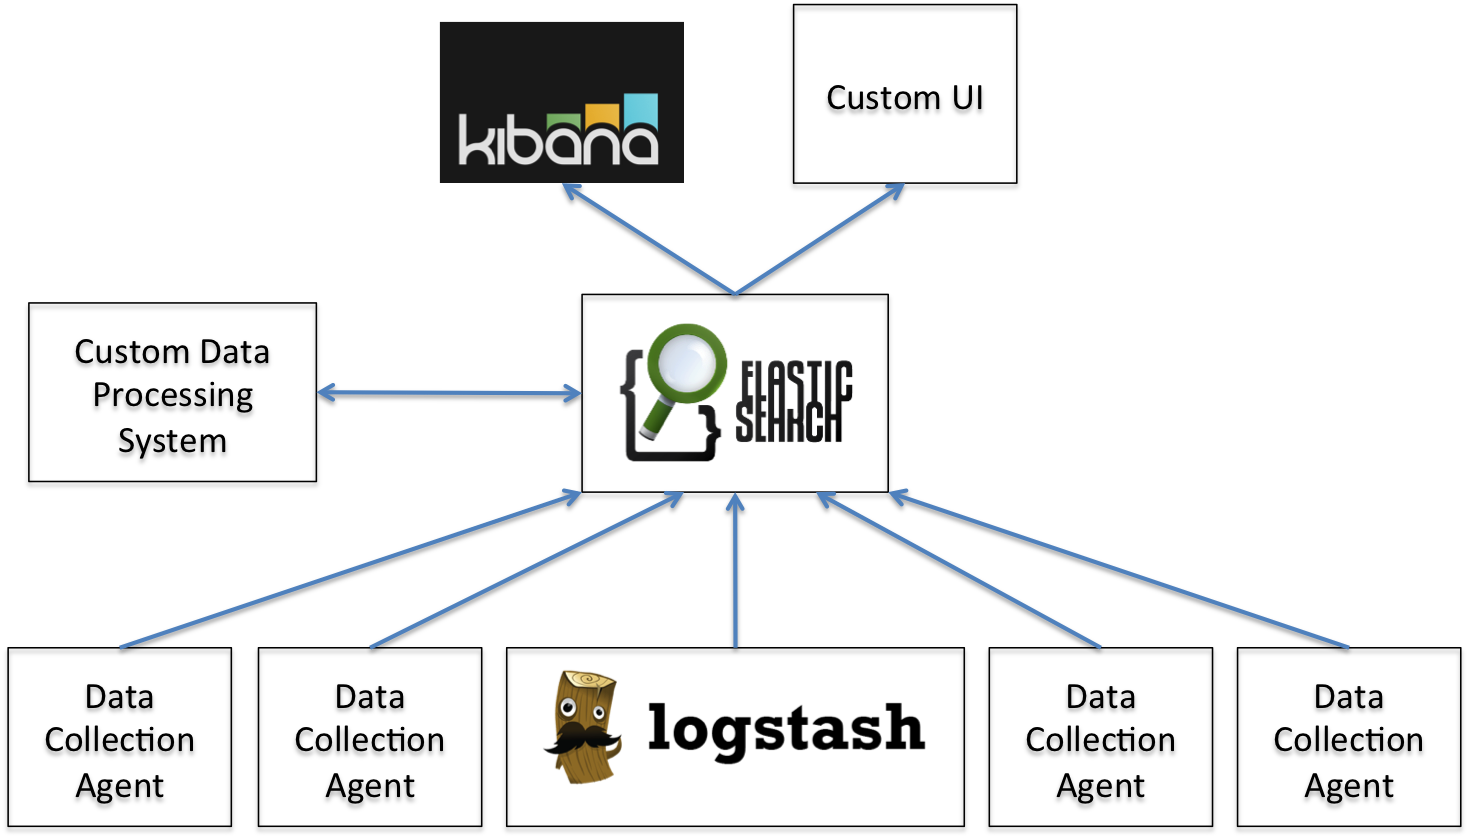
\includegraphics[scale=0.5]{apm_impl}
\caption{APM implementation based on ElasticSearch.}
\label{fig:apm_impl}
\end{figure}

\subsubsection{Data Collection, Storage and Visualization}
In this section we outline some of the technologies and tools that we have chosen to implement the proposed
APM architecture.  After a thorough evaluation of numerous existing system monitoring tools and platforms, 
we have decided to implement our APM for PaaS clouds using ElasticSearch. More specifically, ElasticSearch
will operate as the primary data storage component of the APM. ElasticSearch is ideal for storing large volumes
of structured and semi-structured data. It supports scalability and high availability via sharding and replication.
Perhaps what makes ElasticSearch an excellent choice for an APM is its comprehensive data indexing and
query support. Using the tried and tested Apache Lucene technology, ElasticSearch continuously organizes
and indexes data, making the information available for fast retrieval and efficient querying. 
Additionally it also provides
powerful data filtering and aggregation features, which can greatly simplify the implementations of high-level
data processing algorithms.

Data can be directly stored in ElasticSearch via its REST API. This means most data collection agents can 
simply make HTTP calls to ElasticSearch to add new records. ElasticSearch also supports batch 
processing thereby enabling agents to locally buffer collected data, and store them in batches to avoid
making too many HTTP calls. For scraping server logs and storing the extracted records in ElasticSearch,
we can use the Logstash tool. Logstash supports scraping a wide range of standard log formats (e.g. 
Apache HTTPD access logs), and other custom log formats can be supported via a simple configuration.
It also integrates naturally with ElasticSearch.

For data visualization we are currently considering Kibana, a powerful web-based dash boarding tool 
that is specifically designed to operate in conjunction with ElasticSearch. Kibana provides a wide
range of charting and tabulation capabilities, with particularly strong support for temporal data.  Since
ElasticSearch exposes all stored data via its REST API, it's also possible to bring other visualization
tools into the mix easily.

Figure~\ref{fig:apm_impl} shows the APM deployment view with ElasticSearch and other related technologies
in place. Most of the data processing features are provided by ElasticSearch itself, and other more complex
data analytics can be provided by a custom data processing system.

\subsubsection{Data Analysis}
Roots pods are implemented as standalone Java server processes. Threads are used to run benchmarkers,
anomaly detectors and handlers concurrently within each pod. Pods communicate with ElasticSearch via
REST calls, and most of the data analysis tasks such as filtering and aggregation are performed
at ElasticSearch itself. By doing so most of the heavy computations can be offloaded to the 
ElasticSearch cluster, which is specifically designed for high-performance query processing
and analytics. The pod implementation remains simple, and their runtime overhead is kept
to a minimum.
